\documentclass[11pt]{article}
\usepackage{fullpage,amsmath,amsfonts,mathpazo,microtype,nicefrac,graphicx,verbatimbox,listings,hyperref,enumitem,amssymb,float,fancyhdr}
\DeclareGraphicsExtensions{.pdf,.eps,.png}

% Margins
% \topmargin=-0.45in
% \evensidemargin=0in
% \oddsidemargin=0in
% \textwidth=6.5in
% \textheight=9.0in
% \headsep=0.25in

% \linespread{1.1} % Line spacing

% % Set up the header and footer
% \pagestyle{fancy}
% \lhead{\hmwkAuthorName} % Top left header
% \chead{\hmwkClass\ (\hmwkClassInstructor\ \hmwkClassTime): \hmwkTitle} % Top center header
% \rhead{\firstxmark} % Top right header
% \lfoot{\lastxmark} % Bottom left footer
% \cfoot{} % Bottom center footer
% \rfoot{Page\ \thepage\ of\ \pageref{LastPage}} % Bottom right footer
% \renewcommand\headrulewidth{0.4pt} % Size of the header rule
% \renewcommand\footrulewidth{0.4pt} % Size of the footer rule

% \setlength\parindent{0pt} % Removes all indentation from paragraphs

%----------------------------------------------------------------------------------------
%   TITLE PAGE
%----------------------------------------------------------------------------------------

\title{
\vspace{1cm}
\textmd{\textbf{AC209a Data Science Project: Data Science with User Ratings and Reviews}}\\
% \normalsize\vspace{0.1in}\small{Due\ on\ \hmwkDueDate}\\
% \vspace{0.1in}\large{\textit{\hmwkClassInstructor\ \hmwkClassTime}}
}

\author{\textbf{Andrew Ross, Sophie Hilgard, Reiko Nishihara, Nick Hoernle}}
\date{\today} % Insert date here if you want it to appear below your name

%----------------------------------------------------------------------------------------

\begin{document}

\maketitle

\section*{Data Source}
We downloaded the data from the `Yelp Dataset Challenge' (\url{https://www.yelp.com/dataset_challenge}). The data contains in total 2.7M reviews from 687K users for 86K businesses. Business data consist of 15 features including ID, category of business (e.g., fast food, restaurant, nightlife, etc.), city, full address, operation hours, latitude, longitude, review count, and stars earned. User data consist of 11 features including average stars, compliments, elite, number of fans, IDs of his/her friends, name, review count, vote categories, and the month start a yelp review. 

\section*{Data Exploration}
We here show descriptive summary statistics about the data and results from univariate analyses. 

\begin{figure}[!htb]
\centering
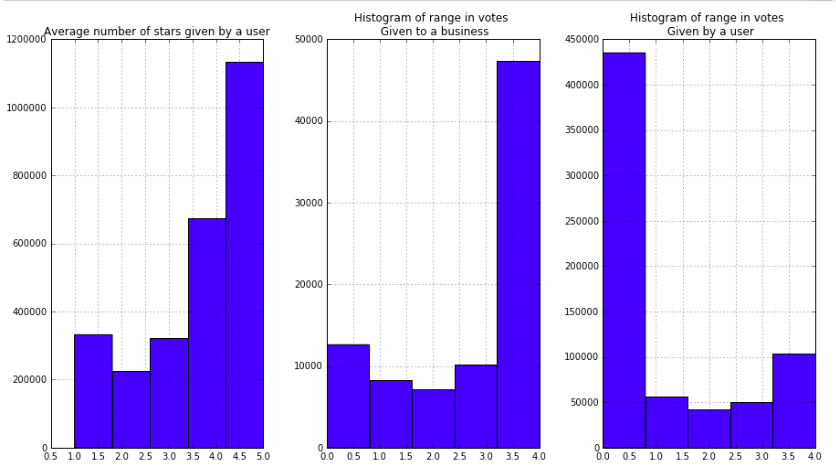
\includegraphics[width=0.9\textwidth]{./ac209/avgstarsusersbusinesses.png}
\end{figure}

\begin{figure}[!htb]
\centering
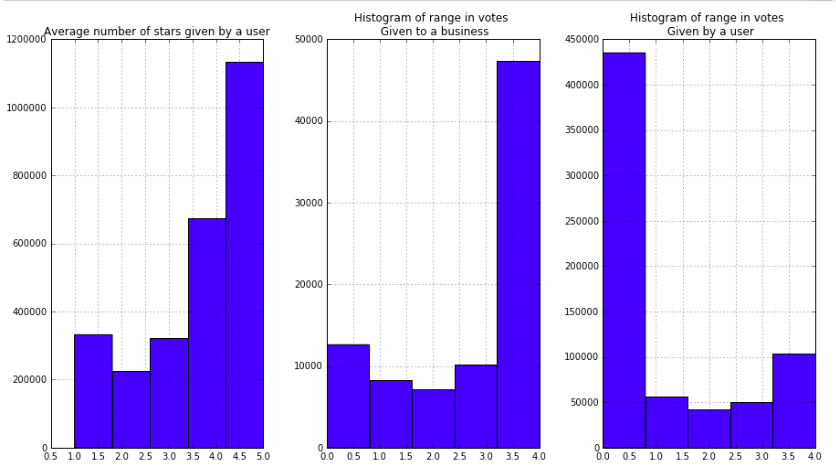
\includegraphics[width=0.9\textwidth]{./ac209/avgstarsusersbusinesses.png}
\end{figure}

\begin{figure}[!htb]
\centering
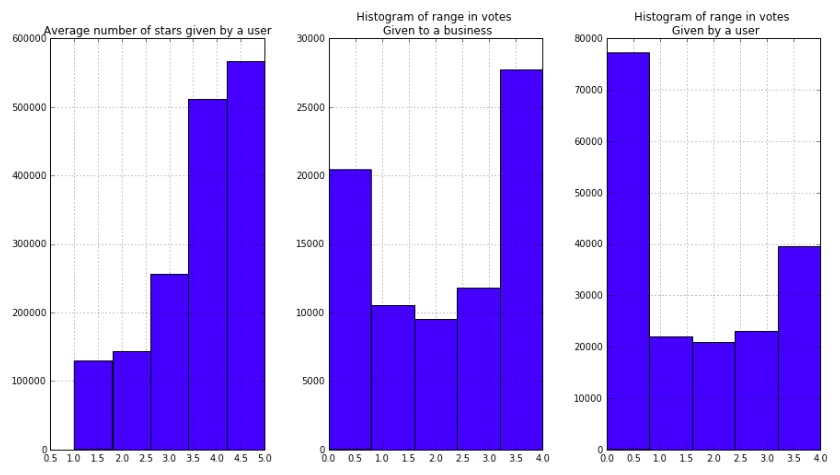
\includegraphics[width=0.9\textwidth]{./ac209/avgstarsusersbusinesses-filter.png}
\end{figure}

\begin{figure}[!htb]
\centering
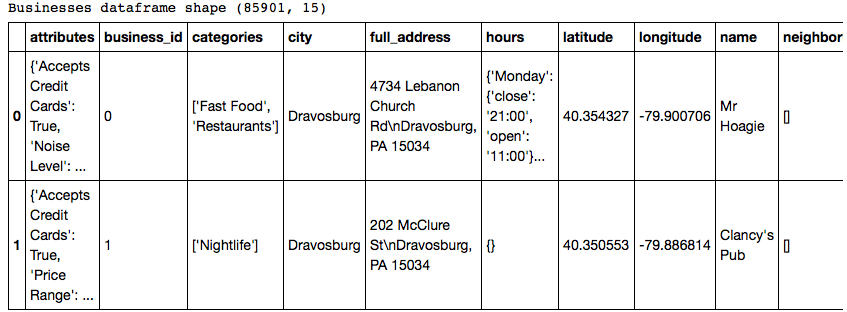
\includegraphics[width=0.9\textwidth]{./ac209/bizdataframe.png}
\end{figure}

\begin{figure}[!htb]
\centering
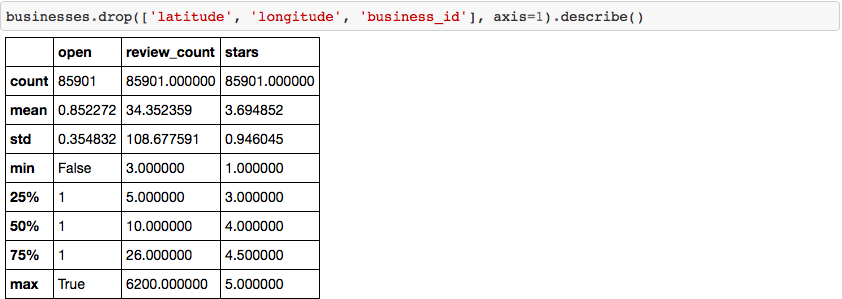
\includegraphics[width=0.9\textwidth]{./ac209/bizdescribe.png}
\end{figure}

\begin{figure}[!htb]
\centering
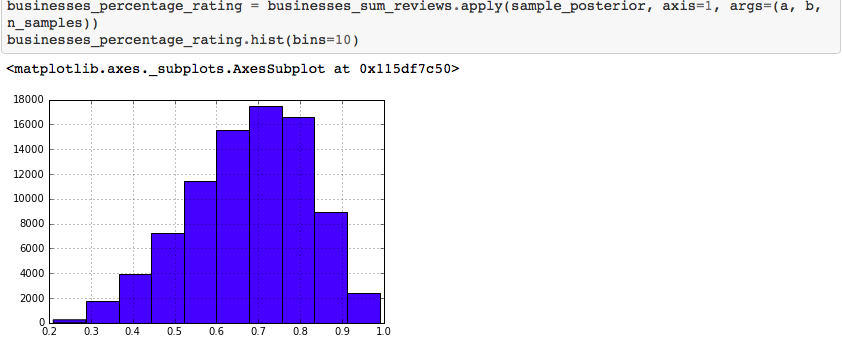
\includegraphics[width=0.9\textwidth]{./ac209/businessespctrating.png}
\end{figure}

\begin{figure}[!htb]
\centering
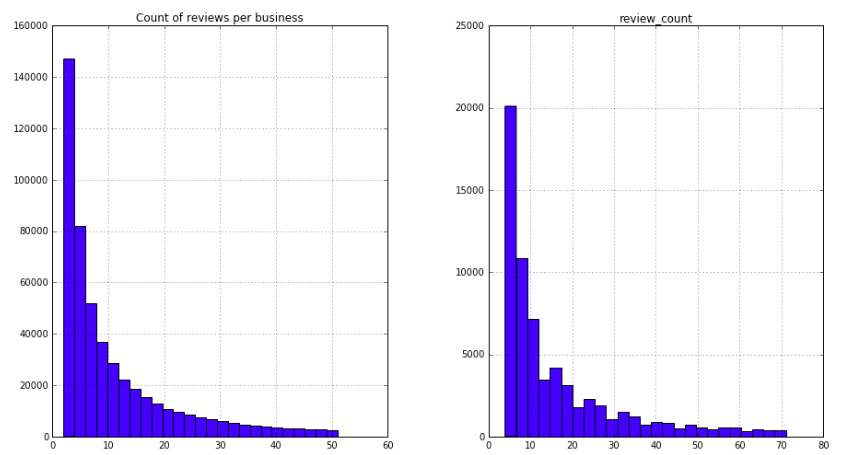
\includegraphics[width=0.9\textwidth]{./ac209/countreviewshist.png}
\end{figure}

\begin{figure}[!htb]
\centering
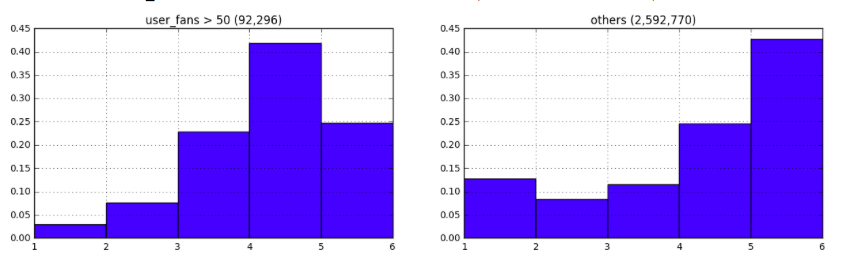
\includegraphics[width=0.9\textwidth]{./ac209/lotsoffans.png}
\end{figure}

\begin{figure}[!htb]
\centering
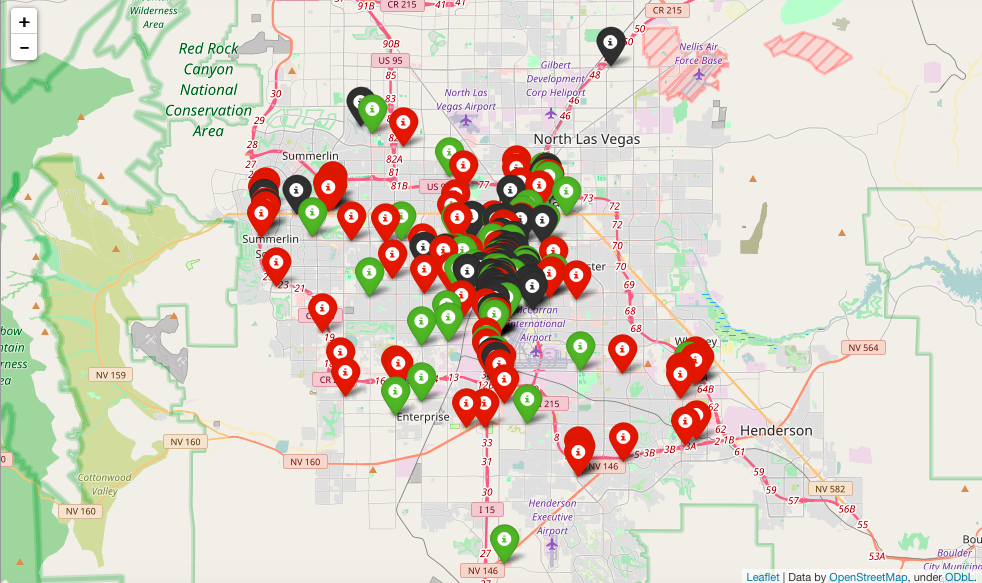
\includegraphics[width=0.9\textwidth]{./ac209/mostreviewsbylocationlv.png}
\end{figure}

\begin{figure}[!htb]
\centering
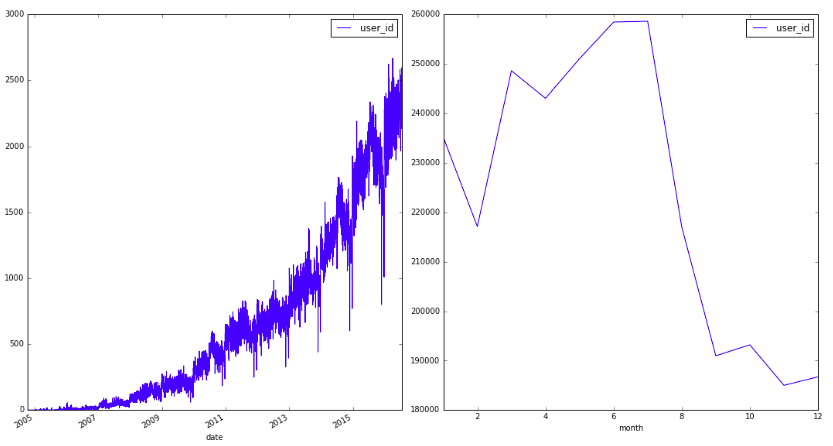
\includegraphics[width=0.9\textwidth]{./ac209/timeseries.png}
\end{figure}

\begin{figure}[!htb]
\centering
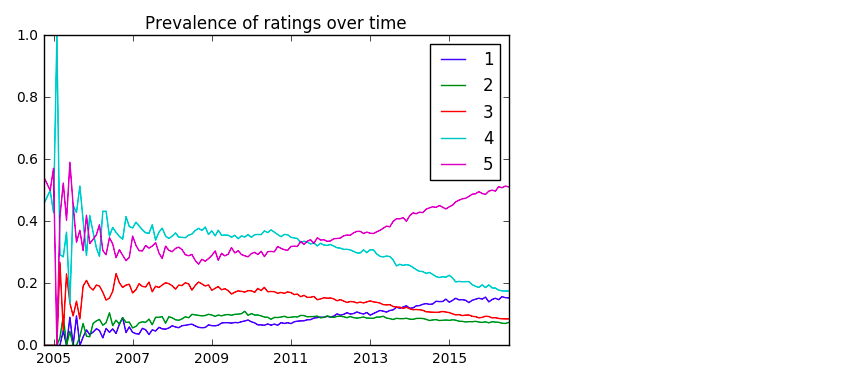
\includegraphics[width=0.9\textwidth]{./ac209/prevalenceofratingsovertime.png}
\end{figure}

\begin{figure}[!htb]
\centering
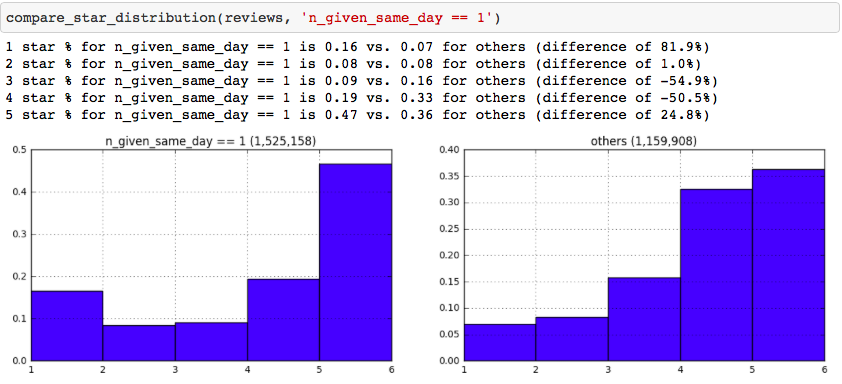
\includegraphics[width=0.9\textwidth]{./ac209/numstarsreviewsperday.png}
\end{figure}

\begin{figure}[!htb]
\centering
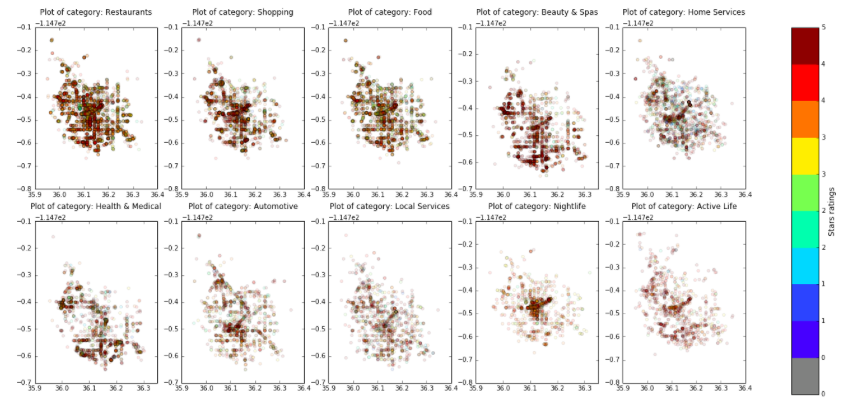
\includegraphics[width=0.9\textwidth]{./ac209/phxstarsbycategorylocation.png}
\end{figure}

\begin{figure}[!htb]
\centering
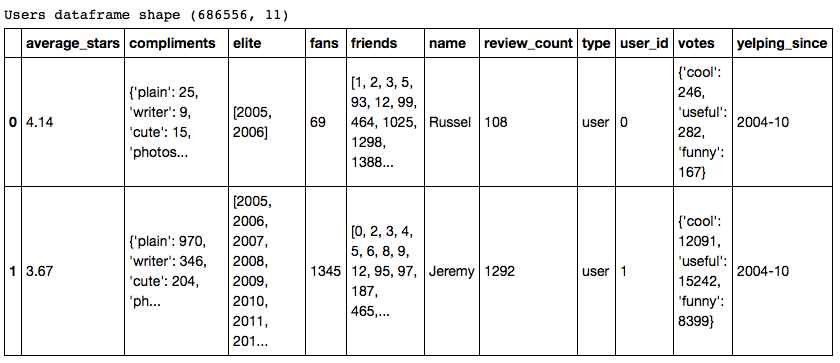
\includegraphics[width=0.9\textwidth]{./ac209/userdataframe.png}
\end{figure}

\begin{figure}[!htb]
\centering
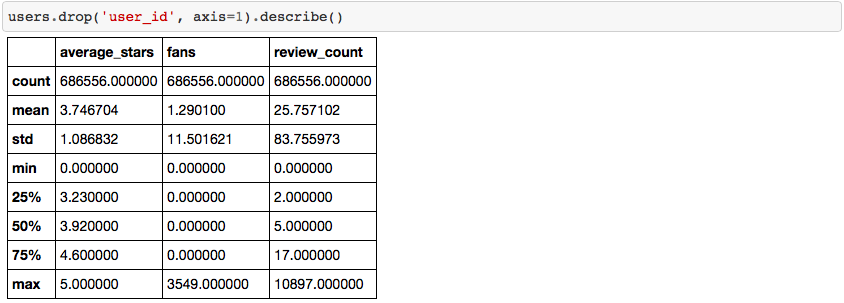
\includegraphics[width=0.9\textwidth]{./ac209/userdescribe.png}
\end{figure}

\begin{figure}[!htb]
\centering
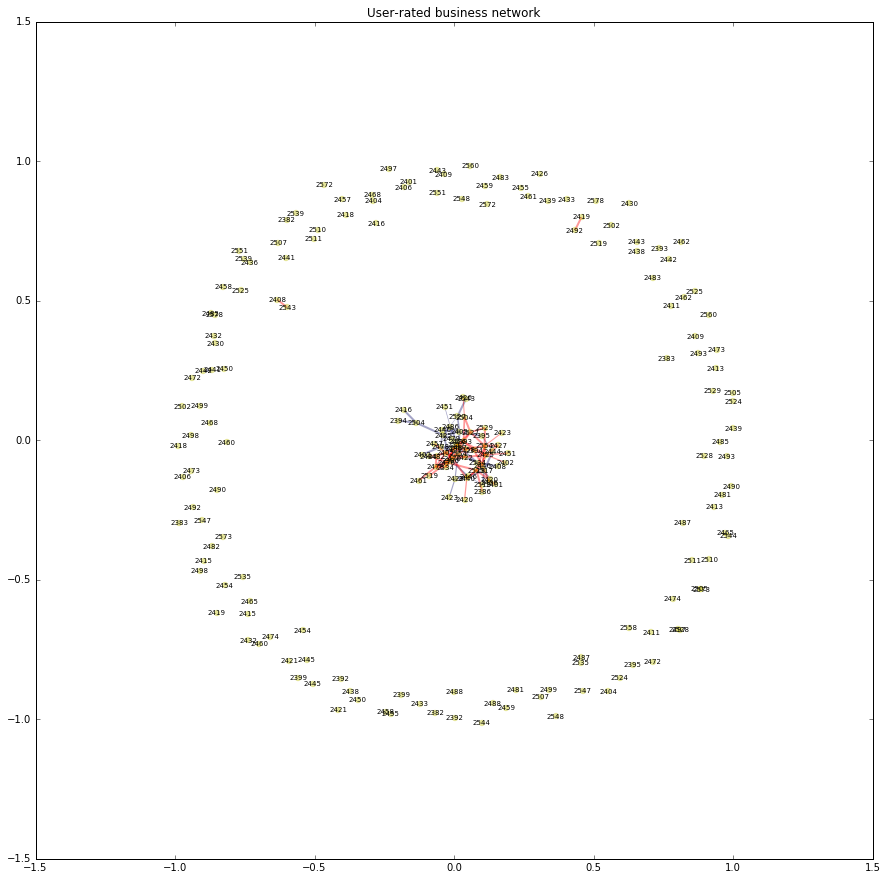
\includegraphics[width=0.9\textwidth]{./ac209/networkanalysis.png}
\end{figure}

\par The table of the users data shows that median value of stars was 3.9 (inter-quartile range, IQR, was 3.2 - 4.6), median value of fans was 0 (IQR, 0 - 0), and median review counts was 5 (IQR, 2 - 17). This indicates that most reviewers do not have fans and wrote a small number of reviews.

\par Figures for the count of reviews per user and count of reviews per business show a unimodal distribution with fatter tail in the right side. Most reviewers tend to write a small number of reviews, and therefore most businesses got a small number of reviews. A question that arises from this plot: for the businesses that receive a high number of ratings, are the ratings more or less positive than the businesses that receive a low number of ratings? The same question can be asked of the users.

\par Now, we plotted average numbers of stars by the number of reviews of users according to the number of reviews in a business. Figures show a modest trend of having higher stars when a business was reviewed by many people. However, we don't see clear relationship among the number of reviews given by a user (or to a business) and the average rating that the business has (or user gives). We can further corroborate this result by analysing the standard deviation in the reviews that a business receives (and a user gives). 

\par We see that users typically rate businesses highly (with a clear mode being 5 stars). However, we also note that businesses have a high range of votes (a mode of 4 indicates that users differ in their opinions). The figure also shows that users did not change their rating schema based on the business, and the majority of users rate all businesses within 1 point of each other. 

\par Using a prior that assumes businesses will not be enjoyed (we wish to overcompensate for the average high ratings of users), we are able to build a more comprehensive likelyhood and thus filter the review somewhat into a more confident top and bottom grouping. The ratings alone are unreliable and we rather wish to include the number of times a business has been rated in a particular manner to calculate the likelihood that this is a favorable (or not) business). For example, if a business is rated poorly twice, this is an unreliable statistic and we do not wish to penalise the business from a median likelihood too dramatically. On the contrary, if a business is rated poorly 100 times, we are confident that users rate the business poorly and we wish to have a low likelihood for enjoyment. In the figure, we show a distribution that corresponds to a probability that this is a good business (i.e., users will like it). On the low end of the scale we have a small number of very poor businesses. We note that these businesses will have a large number of poor ratings. Similarly, on the high end, we see that there is a relatively small number of highly rated businesses. These businesses require a high number of very positive ratings to be rated into this category. We note that we used a fairly aggressive prior assumption that all businesses have a median probability for being liked that is less than 2.5. This is to overcompensate for the generally high ratings. We now have a more normally distributed dataset.

\section*{Time series analysis}
Now, we incorporated time axis on the data and conducted simple analyses. First, we noticed that yelp review has become more popular over time, and possibly, June and July are the most popular months.

\par In earlier years (i.e., before 2008), the average stars varied very widely from 1 to 5 stars. In contrast, after 2009 onward, the average stars converged to around 4. This is mainly because we have more reviews over time and the mean value became less variable. The rating did not differ according to the month reviewed.

\par When we analyzed the number of repeated reviews by a user, we found that majority of reviews reviewed once.

\end{document}

